% !TEX root = ../main.tex
\section{Design Decisions in DSL Development}

\subsection{The Design Problem}

Building a DSL is mostly a series of choices, and the choices interact with each other in
non-obvious ways. Getting the syntax wrong makes the language unreadable. Getting the
semantics wrong makes it unreliable. Getting the execution model wrong makes it slow or
hard to debug. And all of these have to work together.

The fundamental tension is this: the more expressive the language, the harder it is to
implement, analyze, and maintain. The more restricted it is, the less it can express, and
the more frustrated users get when they hit the edges. Every design decision lives on
that spectrum somewhere.

What follows is a breakdown of the main axes, with the training DSL as a running example
for concreteness.

\subsection{Syntax Design}

\subsubsection{The First Question: Who Is Writing This?}

Before deciding anything about syntax, you need to know who your users are. A DSL written
for developers is different from one written for domain experts. Developers tolerate more
syntactic noise (braces, semicolons, type annotations) in exchange for familiar structure.
Domain experts need something that reads like their domain, not like a programming language.

For a training DSL, users are coaches and athletes. The syntax should match the way they
already talk about training, not the way a software engineer would model it.

\subsubsection{Declarative vs Imperative}

The clearest indicator of a well-designed DSL is whether it's declarative. A declarative
program says \emph{what} exists; an imperative program says \emph{what to do}. Compare:

\begin{center}
\begin{tabular}{p{5.5cm}p{5.5cm}}
\hline
\textbf{Declarative (DSL)} & \textbf{Imperative (Python)} \\
\hline
\begin{lstlisting}
Monday:
  run: 10km @threshold
  rest: 15min
\end{lstlisting}
&
\begin{lstlisting}[language=Python]
plan.add_day("Monday")
plan.add_activity(
  "run", 10, "km",
  intensity="threshold"
)
plan.add_activity(
  "rest", 15, "min"
)
\end{lstlisting}
\\
\hline
\end{tabular}
\end{center}

The declarative version doesn't talk about \texttt{add\_day} or \texttt{add\_activity}.
It talks about what the Monday training looks like. That shift in perspective --- from
operations to descriptions --- is what makes a DSL feel natural to a domain expert.

\subsubsection{Verbosity and Conciseness}

There's a direct trade-off between how much you have to write and how easy the language
is to learn. A verbose syntax is more explicit and easier to understand on first read:

\begin{lstlisting}
exercise type=run distance=10 unit=km intensity=threshold
\end{lstlisting}

A concise syntax requires learning the notation but is much faster to write in practice:

\begin{lstlisting}
run: 10km @threshold
\end{lstlisting}

The right choice depends on how often the language gets used. If users write DSL programs
once and read them a hundred times, optimize for readability. If they write dozens of
programs a week, optimize for conciseness. For a training DSL used daily by a coach,
concise wins.

\subsubsection{Whitespace and Structure}

Whether indentation carries meaning is a surprisingly impactful choice. Python and YAML
use indentation as structure, which reads naturally but makes the lexer more complex
(it has to track indent/dedent tokens). JSON and C use explicit delimiters, which are
simpler to parse but add syntactic noise.

For the training DSL, using indentation to separate days from activities is natural --- it
mirrors how a human would write a schedule on paper. The complexity cost of tracking
indentation in the lexer is worth it for the readability gain.

\subsection{Grammar Design}

\subsubsection{Ambiguity Is a Bug}

A grammar is ambiguous when the same input string can be parsed in more than one way.
In a DSL, ambiguity is almost always a mistake --- it means the same program text can be
interpreted as two different things depending on which parse tree the engine picks.

Consider:
\begin{lstlisting}
run 10 km @threshold easy
\end{lstlisting}
Does \texttt{easy} modify the intensity (\texttt{@threshold easy}) or is it a separate
qualifier on the whole activity? Without a clear grammar rule, you can't tell. The parser
will pick one interpretation or fail, and either way the user didn't get what they expected.

Resolution is usually straightforward: require explicit separators, define production
rules carefully, or use different token types for different qualifier kinds. The grammar
should make structure unambiguous, not rely on the user to ``write it right.''

\subsubsection{Context-Free is Usually Enough}

Most DSL syntaxes fit comfortably in the context-free grammar class. Context-free grammars
are parseable in $O(n^3)$ in general, but with LL(1) or LR(1) grammars you get $O(n)$
--- linear time, token by token.

Context-sensitive constraints (``this unit must be compatible with this exercise'') don't
belong in the grammar. They belong in the semantic analysis phase, after the parse tree
is already built. Keeping the grammar context-free makes the parser simple and the error
messages cleaner.

\subsubsection{LL vs LR}

The two main parsing strategies differ in how they build the parse tree:

\begin{description}
  \item[LL(k)] Reads left-to-right, builds a leftmost derivation, uses $k$ tokens of
    lookahead. The grammar must be left-factored (no two rules starting with the same
    token). Straightforward to implement by hand as a recursive-descent parser. Each
    grammar rule becomes a function.
  \item[LR(k)] Reads left-to-right, builds a rightmost derivation in reverse, uses $k$
    tokens of lookahead. Handles more grammars than LL, but the tables are complex to
    build by hand. Generators like Yacc, Bison, and ANTLR do this for you.
\end{description}

For a DSL built by hand (which is almost always the case for small languages), LL(1)
recursive descent is the practical choice. Each production rule maps to a function, error
messages can be precise, and the code is readable. The training DSL grammar is designed
to be LL(1): every rule can be identified by its first token.

\subsubsection{Error Recovery}

A parser that stops at the first error is frustrating. A user should be able to see all
the problems in their program at once, not fix one and re-run to discover the next.

The standard strategy for small DSLs is \emph{panic mode}: when an error is found, skip
tokens until a known synchronization point (a newline, a new day header, a familiar
keyword) and resume parsing from there. It's not perfect, but it gets the job done for
a language where programs are short and errors are local.

Error messages are part of the language's design. A message like:
\begin{lstlisting}
line 3: invalid unit 'min' for exercise 'run'
  expected: 'km' or 'm'
  found: 'min'
\end{lstlisting}
is infinitely more useful than \texttt{parse error at token 'min'}.

\subsection{Architecture of the Interpreter}

The design decisions above converge in the actual implementation. Here's how the
components fit together for an interpreted training DSL:

\begin{center}
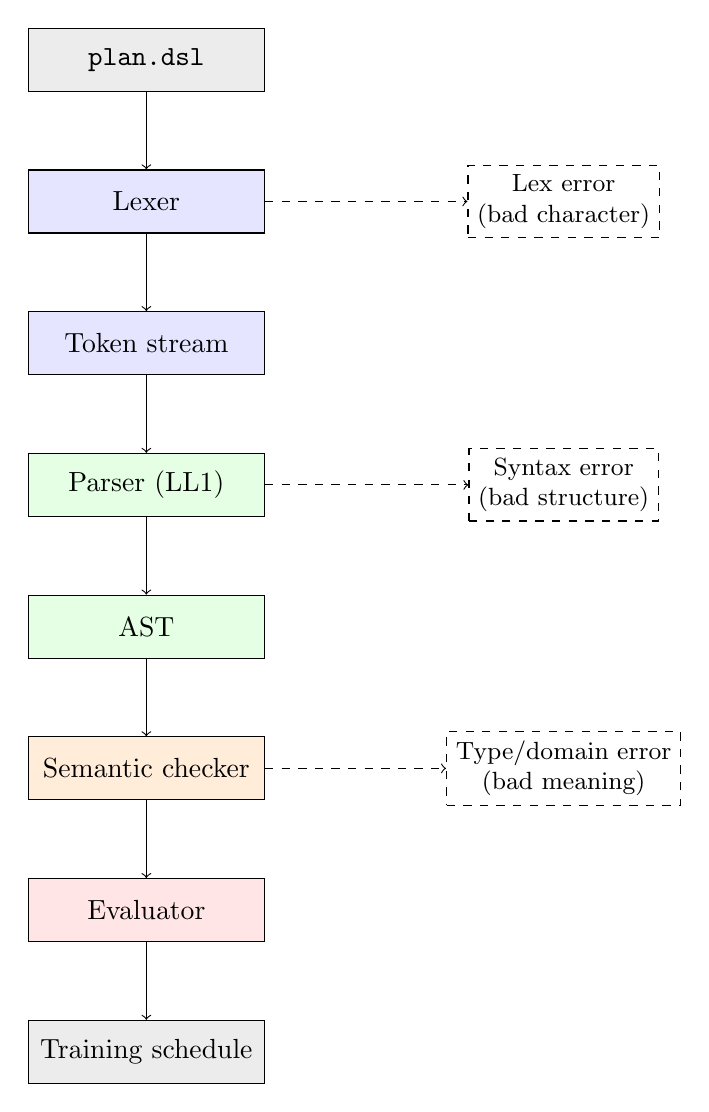
\begin{tikzpicture}[node distance=1.8cm]
  \node (file)   [draw, rectangle, fill=gray!15, minimum width=3cm, minimum height=0.8cm]
                 {\texttt{plan.dsl}};
  \node (lexer)  [draw, rectangle, fill=blue!10, minimum width=3cm, minimum height=0.8cm,
                 below of=file]
                 {Lexer};
  \node (tokens) [draw, rectangle, fill=blue!10, minimum width=3cm, minimum height=0.8cm,
                 below of=lexer]
                 {Token stream};
  \node (parser) [draw, rectangle, fill=green!10, minimum width=3cm, minimum height=0.8cm,
                 below of=tokens]
                 {Parser (LL1)};
  \node (ast)    [draw, rectangle, fill=green!10, minimum width=3cm, minimum height=0.8cm,
                 below of=parser]
                 {AST};
  \node (check)  [draw, rectangle, fill=orange!15, minimum width=3cm, minimum height=0.8cm,
                 below of=ast]
                 {Semantic checker};
  \node (eval)   [draw, rectangle, fill=red!10, minimum width=3cm, minimum height=0.8cm,
                 below of=check]
                 {Evaluator};
  \node (result) [draw, rectangle, fill=gray!15, minimum width=3cm, minimum height=0.8cm,
                 below of=eval]
                 {Training schedule};

  \node (errl) [draw, rectangle, dashed, right of=lexer, xshift=3.5cm,
               font=\small, align=center]
               {Lex error\\(bad character)};
  \node (errp) [draw, rectangle, dashed, right of=parser, xshift=3.5cm,
               font=\small, align=center]
               {Syntax error\\(bad structure)};
  \node (errs) [draw, rectangle, dashed, right of=check, xshift=3.5cm,
               font=\small, align=center]
               {Type/domain error\\(bad meaning)};

  \draw[->] (file)   -- (lexer);
  \draw[->] (lexer)  -- (tokens);
  \draw[->] (tokens) -- (parser);
  \draw[->] (parser) -- (ast);
  \draw[->] (ast)    -- (check);
  \draw[->] (check)  -- (eval);
  \draw[->] (eval)   -- (result);

  \draw[->, dashed] (lexer)  -- (errl);
  \draw[->, dashed] (parser) -- (errp);
  \draw[->, dashed] (check)  -- (errs);
\end{tikzpicture}
\end{center}

Each layer has a single responsibility. The lexer doesn't know about grammar rules. The
parser doesn't know about domain constraints. The semantic checker doesn't know about
execution. This separation makes each component testable independently and makes error
messages precise: you always know which layer caught the problem.

\subsection{Abstraction Level}

One of the harder design decisions is figuring out \emph{how much} to abstract. The right
level is the one that matches the domain's natural vocabulary --- not higher, not lower.

\begin{center}
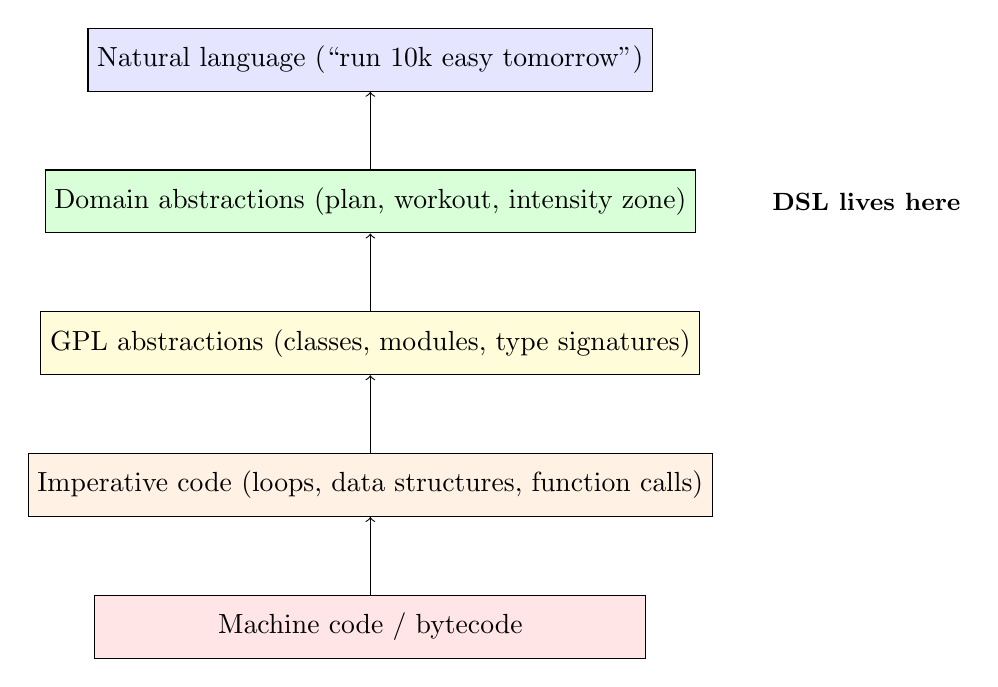
\begin{tikzpicture}[node distance=1.8cm]
  \node (machine) [draw, rectangle, fill=red!10, minimum width=7cm, minimum height=0.8cm]
                  {Machine code / bytecode};
  \node (imperative) [draw, rectangle, fill=orange!10, minimum width=7cm, minimum height=0.8cm,
                     above of=machine]
                     {Imperative code (loops, data structures, function calls)};
  \node (gpl) [draw, rectangle, fill=yellow!15, minimum width=7cm, minimum height=0.8cm,
              above of=imperative]
              {GPL abstractions (classes, modules, type signatures)};
  \node (dsl) [draw, rectangle, fill=green!15, minimum width=7cm, minimum height=0.8cm,
              above of=gpl]
              {Domain abstractions (plan, workout, intensity zone)};
  \node (natural) [draw, rectangle, fill=blue!10, minimum width=7cm, minimum height=0.8cm,
                  above of=dsl]
                  {Natural language (``run 10k easy tomorrow'')};

  \draw[->] (machine)    -- (imperative);
  \draw[->] (imperative) -- (gpl);
  \draw[->] (gpl)        -- (dsl);
  \draw[->] (dsl)        -- (natural);

  \node [right of=dsl, xshift=4.5cm, font=\small, align=left]
        {\textbf{DSL lives here}};
\end{tikzpicture}
\end{center}

Stopping at the GPL layer means the user still has to think like a programmer. Jumping
all the way to natural language means you lose precision and structure (and then you need
an NLP system to translate back). The DSL layer is the sweet spot: structured enough to
be unambiguous and analyzable, but expressive enough to match how the domain expert
thinks.

A \emph{leaky abstraction} happens when the DSL forces the user to think about the layer
below. If a training DSL error message says \texttt{NullPointerException in
ActivityBuilder.java:43}, the abstraction is leaking. The user doesn't know what an
ActivityBuilder is and shouldn't have to.

\subsection{Type System and Domain Constraints}

\subsubsection{Types Prevent Nonsense}

Even a simple type system adds a lot of value. Without one, you can write programs that
are syntactically valid but semantically meaningless:

\begin{lstlisting}
run: 10min     # wrong unit for run
rest: 5km      # duration expected, distance given
intensity: 150% # out of range
\end{lstlisting}

A type system catches these at analysis time, before the program is ever stored or run.

\subsubsection{Type Inference from Context}

For a training DSL, the exercise name determines the expected unit type. \texttt{run}
expects a distance; \texttt{rest} expects a duration. This is type inference: the checker
deduces the required type from context, without the user having to annotate it explicitly.
The user writes \texttt{run: 10km} and the checker knows \texttt{km} is correct because
\texttt{run} has type signature $\text{Distance} \to \text{Activity}$.

\subsubsection{Domain Constraints as Refinement Types}

Some constraints go beyond simple types. You can encode them as refinement types --- types
with predicates:
\[
  \text{Distance} = \{ d : \mathbb{R} \mid d > 0 \}
  \qquad
  \text{Intensity} = \{ i : \mathbb{R} \mid 0 < i \leq 1 \}
\]

A value like $d = -5$ fails the predicate and gets rejected at analysis time. You don't
need to add runtime checks in the evaluator because the semantic checker already guarantees
all values are valid before execution starts. This is the ``correctness by construction''
argument for DSLs.

\subsubsection{Static vs Dynamic Checking}

Static checking (at analysis time) is always better for a language where programs are
stored and re-used. A training plan that was valid when it was written should still be
valid six months later. Dynamic checking (at runtime) defers that guarantee until the
program actually runs, which is too late if the program is sitting in a database.

The rule for a training DSL is simple: if it's wrong, reject it before it gets stored.

\subsection{Semantic Design}

\subsubsection{Operational Semantics}

An operational semantics defines meaning by giving reduction rules. For the training DSL,
small-step rules build up the schedule state $\sigma$:

\[
  \frac{a = \text{Activity}(\text{run},\; d,\; u)}
       {\langle \texttt{run:}\; d\,u,\; \sigma \rangle \;\to\;
        \langle \text{done},\; \sigma[\text{activities} \mathrel{+}= a] \rangle}
\]

This is useful for implementors because it tells you exactly how the evaluator should
behave, step by step.

\subsubsection{Denotational Semantics}

The denotational approach defines a function that maps programs to mathematical values
directly. For the training DSL:
\[
  \llbracket \text{plan} \rrbracket = \{ \llbracket d \rrbracket \mid d \in \text{days}(\text{plan}) \}
\]
\[
  \llbracket \texttt{run: 10km @threshold} \rrbracket =
  \text{Activity}(\text{run},\; 10,\; \text{km},\; \text{threshold})
\]

This style is useful for reasoning about whether two programs are equivalent --- if
$\llbracket p_1 \rrbracket = \llbracket p_2 \rrbracket$, the programs mean the same thing
even if they look different syntactically.

\subsection{Execution Model Choices}

\subsubsection{Interpretation vs Compilation}

For a DSL, interpretation is almost always the right starting point. You walk the AST
and produce results directly. No build step, no generated code to debug, errors can point
directly to source locations. The training DSL has no performance requirements that would
justify compilation.

\begin{center}
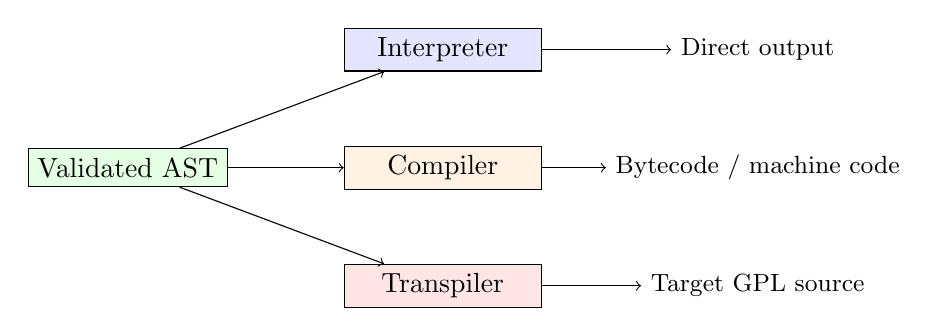
\begin{tikzpicture}[node distance=2.5cm]
  \node (ast) [draw, rectangle, fill=green!10, minimum width=2.5cm]
              {Validated AST};

  \node (interp) [draw, rectangle, fill=blue!10, minimum width=2.5cm,
                 right of=ast, xshift=1.5cm, yshift=1.5cm]
                 {Interpreter};
  \node (comp)   [draw, rectangle, fill=orange!10, minimum width=2.5cm,
                 right of=ast, xshift=1.5cm]
                 {Compiler};
  \node (transp) [draw, rectangle, fill=red!10, minimum width=2.5cm,
                 right of=ast, xshift=1.5cm, yshift=-1.5cm]
                 {Transpiler};

  \node (r1) [right of=interp, xshift=1.5cm, font=\small] {Direct output};
  \node (r2) [right of=comp,   xshift=1.5cm, font=\small] {Bytecode / machine code};
  \node (r3) [right of=transp, xshift=1.5cm, font=\small] {Target GPL source};

  \draw[->] (ast) -- (interp);
  \draw[->] (ast) -- (comp);
  \draw[->] (ast) -- (transp);
  \draw[->] (interp) -- (r1);
  \draw[->] (comp)   -- (r2);
  \draw[->] (transp) -- (r3);
\end{tikzpicture}
\end{center}

Compilation makes sense when performance is critical and the domain involves computation
(like a numerical simulation DSL). Transpilation makes sense when you want to integrate
with an existing ecosystem (like TypeScript transpiling to JavaScript). For a training
DSL that produces schedules and statistics, interpretation is the right model.

\subsection{Error Handling as a First-Class Feature}

Error handling is not something you add at the end. It's part of the language design.

The four levels of errors in a DSL form a hierarchy:

\begin{enumerate}
  \item \textbf{Lexical errors} --- something the lexer doesn't recognize.
    \texttt{r\%n: 10km} fails because \texttt{\%} isn't in the alphabet.
  \item \textbf{Syntax errors} --- valid tokens in an invalid structure.
    \texttt{run 10km:} fails because the colon is in the wrong position.
  \item \textbf{Semantic errors} --- valid structure, wrong types or constraints.
    \texttt{run: 10min} fails because \texttt{min} is a duration unit, not a distance.
  \item \textbf{Domain errors} --- valid and typed, but physically unreasonable.
    \texttt{run: 500km @sprint} passes all structural checks but represents an impossible
    training session.
\end{enumerate}

Each level requires a different kind of check, and each should produce a different kind
of message. The key principle is: \emph{every error message should tell the user what
went wrong, where it went wrong, and what would have been correct}. A domain-specific
language should produce domain-specific errors.

\subsection{The AI Integration Layer}

One distinctive design decision for this particular DSL is the integration with an AI
layer. The system accepts natural language input (``add a threshold run Monday, about
10k'') and translates it into a valid DSL program before parsing. This is not part of
the DSL itself --- it's a translation layer that sits in front of the lexer.

\begin{center}
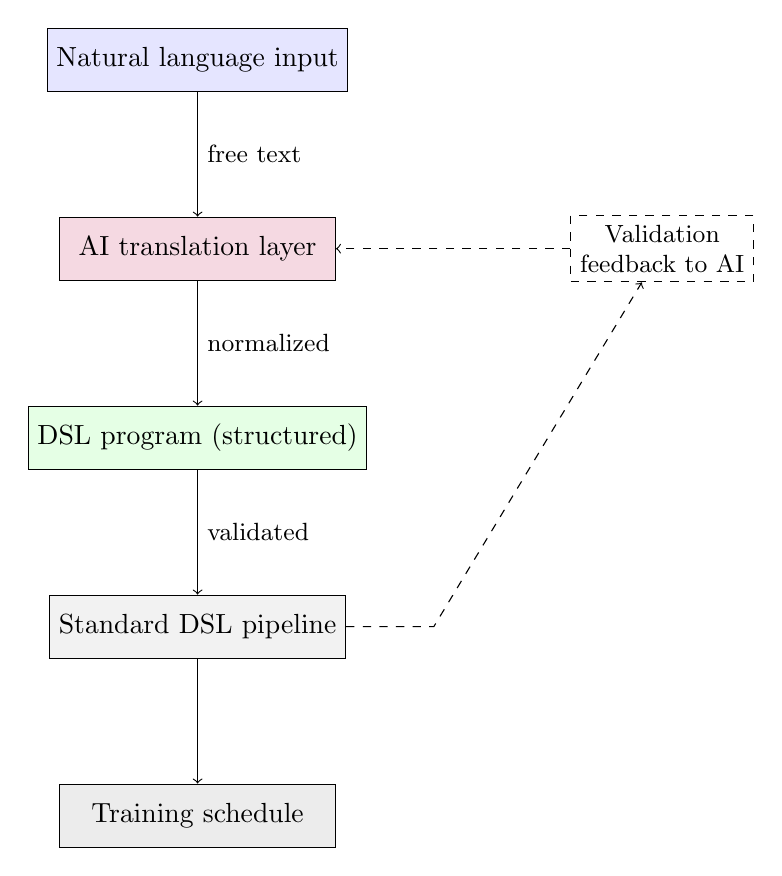
\begin{tikzpicture}[node distance=2.4cm]
  \node (nl)   [draw, rectangle, fill=blue!10, minimum width=3.5cm, minimum height=0.8cm]
               {Natural language input};
  \node (ai)   [draw, rectangle, fill=purple!15, minimum width=3.5cm, minimum height=0.8cm,
               below of=nl]
               {AI translation layer};
  \node (dsl)  [draw, rectangle, fill=green!10, minimum width=3.5cm, minimum height=0.8cm,
               below of=ai]
               {DSL program (structured)};
  \node (pipe) [draw, rectangle, fill=gray!10, minimum width=3.5cm, minimum height=0.8cm,
               below of=dsl]
               {Standard DSL pipeline};
  \node (out)  [draw, rectangle, fill=gray!15, minimum width=3.5cm, minimum height=0.8cm,
               below of=pipe]
               {Training schedule};

  \draw[->] (nl)   -- (ai)   node[midway, right, font=\small] {free text};
  \draw[->] (ai)   -- (dsl)  node[midway, right, font=\small] {normalized};
  \draw[->] (dsl)  -- (pipe) node[midway, right, font=\small] {validated};
  \draw[->] (pipe) -- (out);

  \node (feedback) [draw, rectangle, dashed, right of=ai, xshift=3.5cm,
                   font=\small, align=center]
                   {Validation\\feedback to AI};
  \draw[->, dashed] (pipe) -- ++(3,0) -- (feedback);
  \draw[->, dashed] (feedback) -- (ai);
\end{tikzpicture}
\end{center}

The reason this architecture makes sense is that the DSL acts as a \emph{structured
intermediate representation}. The AI doesn't output training schedules directly --- it
outputs DSL programs that are then validated by the full pipeline. If the AI produces
something invalid (wrong unit, impossible value, malformed structure), the semantic
checker catches it. The validation feedback can even be fed back to the AI to ask for
a correction.

This separation is important: the AI handles the ambiguity and variability of natural
language; the DSL handles correctness and structure. Trying to do both in the same
component would make both worse.

\subsection{Extensibility and Evolution}

A DSL that can't evolve without breaking existing programs is a liability. The most
important extensibility rule is: \emph{new features should be additive}. Adding a new
exercise type, a new optional qualifier, or a new top-level concept should not invalidate
old programs.

\begin{itemize}
  \item New terminals (new exercise types) can be added to the grammar without structural
    changes.
  \item New optional constructs don't affect programs that don't use them.
  \item New required constructs are breaking changes and need versioning.
\end{itemize}

For long-lived DSLs, explicit version headers (\texttt{version: 2}) let the parser decide
which grammar to apply. For a DSL early in development, keeping changes additive is usually
enough.

\subsection{Summary: Design Decisions for the Training DSL}

Every decision described above has a concrete answer for the training DSL:

\begin{center}
\begin{tabular}{p{4cm}p{3cm}p{5cm}}
\hline
\textbf{Decision} & \textbf{Choice} & \textbf{Reason} \\
\hline
Style             & Declarative   & Matches how coaches think \\
Syntax            & Concise       & Used daily by the same users \\
Structure         & Indentation   & Natural schedule layout \\
Parser            & LL(1) by hand & Small grammar, precise errors \\
Type checking     & Inferred, static & Concise syntax + early error detection \\
Execution         & Interpreted   & No performance requirement \\
Error messages    & Domain-level  & Users are not programmers \\
AI integration    & Separate layer & Keeps DSL semantics clean \\
Evolution         & Additive      & Don't break stored plans \\
\hline
\end{tabular}
\end{center}

The through-line across all these decisions is the same: the design serves the user, not
the implementor. A training DSL that forces a coach to think about parsers or type systems
has failed. The goal is for the language to disappear --- for the user to think about
training, not syntax.
